\documentclass[11pt]{article}
\usepackage{graphicx}
\setlength{\topmargin}{0.0in}
\setlength{\oddsidemargin}{-0.05in}
\setlength{\evensidemargin}{-0.05in}
\setlength{\textheight}{8.5in}
\setlength{\textwidth}{6.5in}
\setlength{\marginparwidth}{0.0in}
\setlength{\marginparsep}{0.0in}
\setlength{\marginparpush}{0.0in}


%%% Libraries added
\usepackage{amsmath}
\usepackage{amssymb}
\usepackage{textcomp,gensymb}

\renewcommand{\thefootnote}{\fnsymbol{footnote}}
\newcounter{temp}
\setcounter{temp}{2}
\setcounter{footnote}{1}
\renewcommand{\thetemp}{\fnsymbol{temp}}
\renewcommand{\thesection}{\Roman{section}}
\renewcommand{\thesubsection}{\thesection-\Alph{subsection}}
\newcommand{\beq}{\begin{equation}}
\newcommand{\eeq}{\end{equation}}
\newcommand{\be}{\begin{enumerate}}
\newcommand{\ee}{\end{enumerate}}
\newcommand{\bea}{\begin{eqnarray}}
\newcommand{\eea}{\end{eqnarray}}
\newcommand{\denotes}{\stackrel{\triangle}{=}}

% Executing solutions
\newif\ifsolutions
\solutionsfalse


\begin{document}

\input{epsf}
\vspace*{-1in}
\begin{center}
\Large
{{\bf ECEN 314: Signals and Systems - Homework 1}}
\end{center}
\begin{itemize}
\item Date Assigned:  Monday 08/31/2021
\item Date Due: Wednesday, 09/07/2021
\end{itemize}
\hrule

\section{Reading Exercise}
Notes on mathematical preliminaries
\section{Problems}
\begin{enumerate}
\item Express each of the following complex numbers in polar form and plot them in the complex plane, indicating the magnitude and angle (or, phase) of each complex number
    \begin{itemize}
    \item[(a)] $(\sqrt{3}+j^3)(1-j)$
    \item[(b)] $ \frac{2-j(6/\sqrt{3})}{2+j(6/\sqrt{3})}$
    \item[(c)] $(\sqrt{3}+j) \ 2\sqrt{2} \ e^{-j\pi/4}$
    \end{itemize}

\ifsolutions
\begin{flalign*}
& \text{Solution :} &
\end{flalign*}
\vspace{-25pt}
\begin{flalign*}
& \text{Problem 1 a)} &
\end{flalign*}
\vspace{-45pt}


\begin{flalign*}
(\sqrt{3}+j^3)(1-j) & =(\sqrt{3}-j)(1-j)\ \ [\text{since}\  j^3=j^2 \times j=(-1)\times j] &\\
& = (\sqrt{3}-\sqrt{3}j-j-1) &\\
& = (-1 + \sqrt{3}) + j(-1-\sqrt{3}) &
\end{flalign*}

\vspace{-15pt}


\begin{flalign*}
\text{Magnitude} & = \sqrt{(-1+\sqrt{3})^2 + (-1 - \sqrt{3})^2} &\\
 & = \sqrt{(1-2\sqrt{3}+3) + (1+2\sqrt{3}+3)} \ \  [(a+b)^2=(a^2+2ab+b^2)] &\\
 & = \sqrt{2+6}\ = \ \sqrt{8}\ =\ 2\sqrt{2} &
\end{flalign*}

\vspace{-15pt}
\begin{flalign*}
& \text{angle or phase}  = \text{tan}^{-1}{\frac{(-1-\sqrt{3})}{(-1+\sqrt{3})}}= -75^{\circ} &\\
\end{flalign*}

\begin{figure}[h]
\centering

\includegraphics[width=12cm]{q1_a.jpg}
\caption{Problem 1 a)}
\end{figure}


% problem 1b

\begin{flalign*}
& \text{Problem 1 b)} &
\end{flalign*}

\vspace{-15pt}

\begin{flalign*}
\frac{2-j(6/\sqrt{3})}{2+j(6/\sqrt{3})} & = \frac{(2-j(6/\sqrt{3}))^2}{(2+j(6/\sqrt{3}))(2-j(6/\sqrt{3}))} &\\
& = \frac{4-j(\frac{24}{\sqrt{3}})-\frac{36}{3}}{4+\frac{36}{3}} = \frac{-8-j8\sqrt{3}}{16} &\\
& = - \frac{1}{2} - j\frac{\sqrt{3}}{2}  &
\end{flalign*}

\vspace{-15pt}

\begin{flalign*}
\text{magnitude} &= \sqrt{(\frac{1}{2})^2 + (\frac{\sqrt{3}}{2})^2} &\\
& = \sqrt{\frac{1}{4} + \frac{3}{4}}=\ 1 & \\
\text{angle} &= \text{tan}^{-1}{(\frac{-\frac{\sqrt{3}}{2}}{-\frac{1}{2}})} = 240^{\circ} &
\end{flalign*}

\begin{figure}[h]
\centering
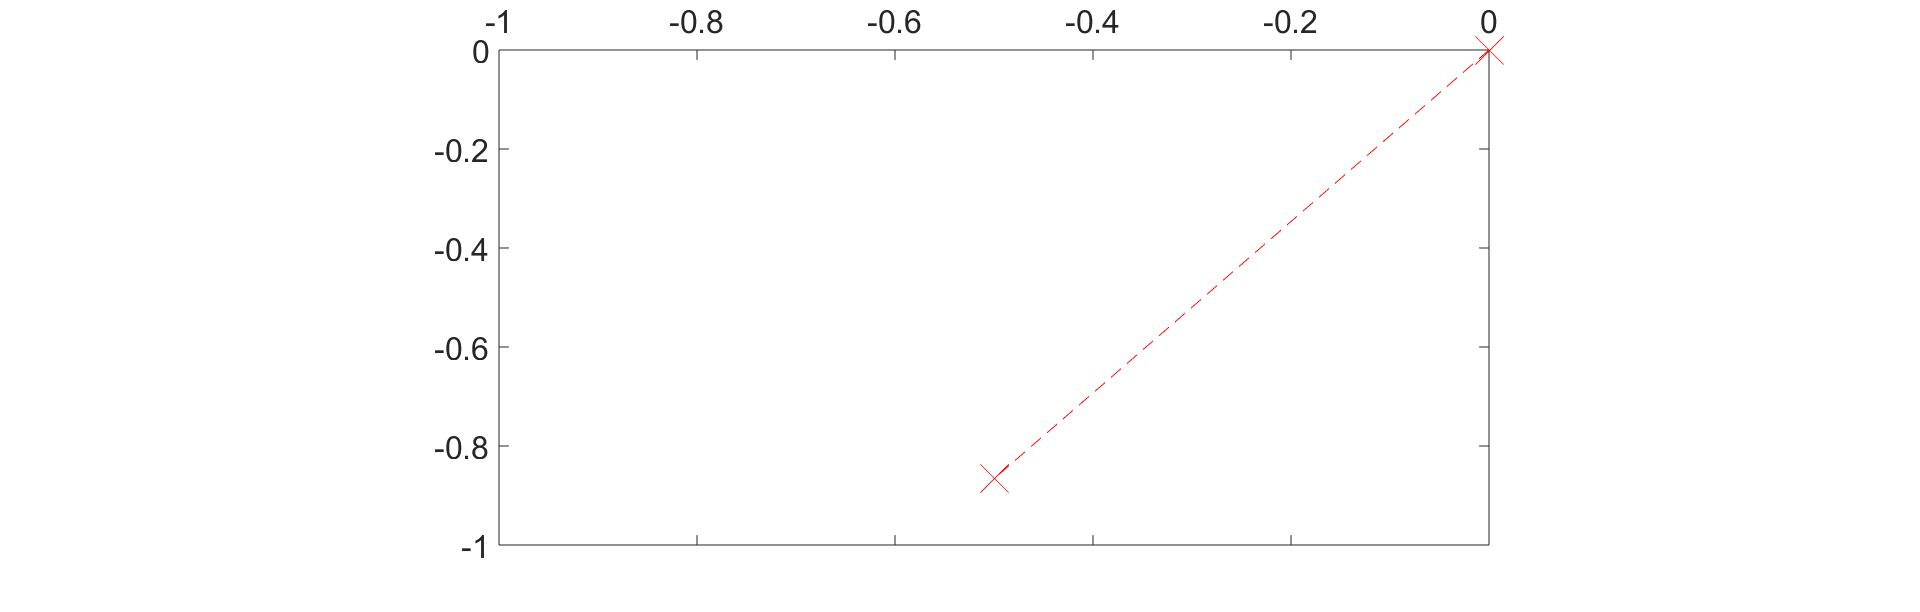
\includegraphics[width=12cm]{q1_b.jpg}
\caption{Problem 1 b)}
\end{figure}

% solution 1c
\begin{flalign*}
& \text{Problem 1 c)} &
\end{flalign*}

\vspace{-15pt}

\begin{flalign*}
&(\sqrt{3}+j)2\sqrt{2}e^{-j\frac{\pi}{4}}= (2\sqrt{6}+j2\sqrt{2})e^{-j \frac{\pi}{4}}&\\
&|2\sqrt{6}+j2\sqrt{2}| =\sqrt{4 \cdot 6 + 4 \cdot 2}=\sqrt{24 + 8} = \sqrt{32}= 2\sqrt{8}= 4\sqrt{2} &\\
&\measuredangle{(2\sqrt{6}+j2\sqrt{2})}= \text{tan}^{-1}{(\frac{2\sqrt{2}}{2\sqrt{6}})} = \text{tan}^{-1}{(\frac{1}{\sqrt{3}})}=\frac{\pi}{6}&\\
&(2\sqrt{6}+j2\sqrt{2})e^{-j \frac{\pi}{4}} = 4\sqrt{2}e^{j\frac{\pi}{6}}e^{-j\frac{\pi}{4}}=4\sqrt{2}e^{-j\frac{\pi}{12}}&\\
&\text{Hence, magnitude} = 4\sqrt{2}&\\
&\measuredangle{ }= -\frac{\pi}{12} = -15^{\circ}&\\
%&(\sqrt{3}+j)2\sqrt{2}e^{-j\frac{\pi}{4}}=4\sqrt{2}e^{\frac{\pi}{12}}=4\sqrt{2}\cos{\frac{\pi}{12}} + 4\sqrt{2}\sin{\frac{\pi}{12}}=5.4641 + j1.4641 &
\end{flalign*}


\begin{figure}[h]
\centering
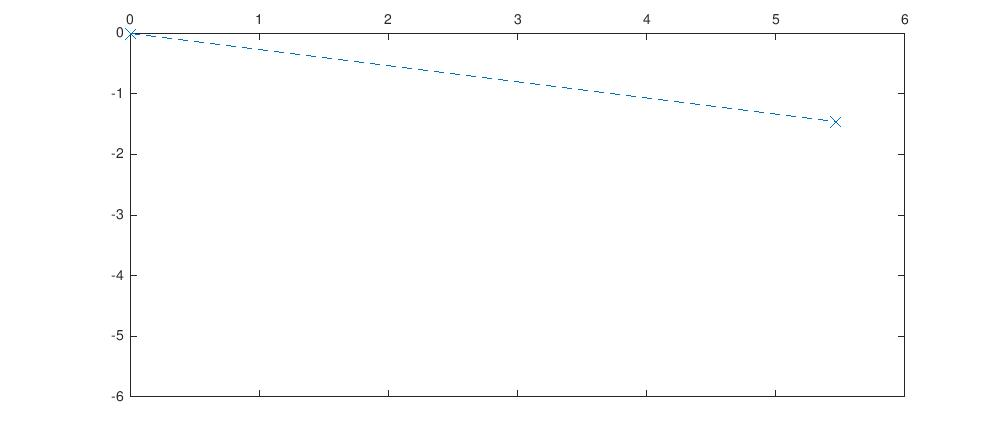
\includegraphics[width=12cm]{q1_c.jpg}
\caption{Problem 1 c)}
\end{figure}

\fi

% question 2

\item Using Euler's relation, derive the following relationships.
    \begin{itemize}
    \item[(a)] $\cos^2 \theta = \frac{1}{2} (1 + \cos 2 \theta)$
    \item[(b)] $\sin\theta \ \sin\phi = \frac{1}{2}\cos(\theta-\phi) - \frac{1}{2}\cos(\theta+\phi)$
    \end{itemize}


\ifsolutions
% solution 2
\begin{flalign*}
& \text{Solution :} &
\end{flalign*}
\vspace{-25pt}
\begin{flalign*}
& \text{Problem 2 a)} &
\end{flalign*}

\vspace{-35pt}

\begin{flalign*}
& \text{prove:} \cos^2{\theta}= \frac{1}{2}(1+\cos{2\theta}) &
\end{flalign*}

\vspace{-15pt}

\begin{flalign*}
\cos^2{\theta} &= (\frac{1}{2} (e^{j\theta} + e^{-j\theta}))^2 = \frac{1}{4}(e^{2j\theta}+2e^{j\theta}e^{-j\theta}+e^{-2j\theta}) &\\
 &= \frac{1}{4}(2+e^{2j\theta}+e^{-2j\theta}) = \frac{1}{4}(2+2\cos{2\theta})  &\\
 &= \frac{1}{2}(1+\cos{\theta})
\end{flalign*}


\begin{flalign*}
& \text{Problem 2 b)} &
\end{flalign*}

\vspace{-35pt}

\begin{flalign*}
& \text{prove}: \sin{\theta}\sin{\phi}= \frac{1}{2} \cos{(\theta-\phi)}-\frac{1}{2} \cos{(\theta+\phi)}&\\
&\text{Proof}:
\end{flalign*}

\vspace{-15pt}

\begin{flalign*}
\sin{\theta}\sin{\phi} &= \frac{1}{2j}(e^{j\theta}-e^{-j\theta}) \frac{1}{2j}(e^{j\phi}-e^{-j\phi})&\\
&= \frac{-1}{4}(e^{j\theta}-e^{-j\theta})(e^{j\phi}-e^{-j\phi}) &\\
&= \frac{-1}{4}(e^{j(\theta+\phi)}-e^{j(\theta-\phi)}-e^{-j(\theta-\phi)}+e^{-j(\theta+\phi)}) &\\
&= \frac{-1}{4}(\{e^{j(\theta+\phi)}+e^{-j(\theta+\phi)}\}-\{e^{j(\theta-\phi)}+e^{-j(\theta-\phi)}\}) &\\
&= \frac{-1}{4}(2\cos{(\theta+\phi)}-2\cos{(\theta-\phi)})&\\
&= \frac{1}{2}(\cos{(\theta-\phi)}-\cos{(\theta+\phi)})
\end{flalign*}

\fi

% question 3

\item Derive the following relations where $z,z_1$ and $z_2$ are arbitrary complex numbers.
    \begin{itemize}
    \item[(a)] $(e^z)^* = e^{z^*}$
    \item[(b)] $z_1 z_2^* + z_1^* z_2 = 2 \Re\{(z_1 z_2^*)\} = 2 \Re\{z_1^* z_2\}$
    \item[(c)] $|z_1 z_2^* + z_1^* z_2| \leq 2 |z_1 z_2|$
    \end{itemize}

\ifsolutions
%solution
\begin{flalign*}
& \text{Solution :} &
\end{flalign*}
\vspace{-25pt}
\begin{flalign*}
& \text{Problem 3 a)} &
\end{flalign*}

\vspace{-15pt}

\begin{flalign*}
&{(e^{z})}^{*} = {(e^{z^{*}})}&
\end{flalign*}

\vspace{-15pt}
\begin{flalign*}
\text{Proof:}\\
e^{z}&=e^{a+jb}=e^{a}(\cos{(b)}+j\sin{(b)})&\\
{(e^{z})}^{*}&=e^{a}{(\cos{(b)}+j\sin{(b)})}^{*} = e^{a}(\cos{(b)}-j\sin{(b)})=e^{a}(\cos{(-b)}+j\sin{(-b)}) &\\
&= e^{a}e^{-jb}=e^{a-jb}=e^{{(a+jb)}^{*}}= e^{z^{*}} &
\end{flalign*}


\begin{flalign*}
& \text{Problem 3 b)} &
\end{flalign*}

\vspace{-15pt}

\begin{flalign*}
& z_{1}{z_{2}}^{*} + {z_{1}}^{*}{z_{2}} = 2R{(z_{1}{z_{2}}^{*})} &
\end{flalign*}

\vspace{-15pt}

\begin{flalign*}
& \text{Proof:} &\\
& \text{Let}\ \  r_{1}= magnitude(z_1), \ \ \theta_1= \measuredangle{z_1}, \ \ r_{2}= magnitude(z_2), \ \ \theta_2= \measuredangle{z_2} &
\end{flalign*}

\vspace{-15pt}

\begin{flalign*}
z_{1}{z_{2}}^{*} + {z_{1}}^{*}{z_{2}} &= r_1 r_2 e^{j(\theta_1 - \theta_2)} + r_1 r_2 e^{-j(\theta_1 - \theta_2)} &\\
&= 2 r_1 r_2 \cos{(\theta_1 - \theta_2)} &
\end{flalign*}

\vspace{-15pt}

\begin{flalign*}
2 Re\{z_{1}{z_{2}}^{*}\} &= 2 Re\{r_1 r_2 e^{j(\theta_1 - \theta_2)}\}  &\\
&= 2 Re \{r_1 r_2 (\cos{(\theta_1 - \theta_2)}+j \sin{(\theta_1 - \theta_2)}) \} &\\
&= 2 r_1 r_2 (\cos{(\theta_1 - \theta_2)}) &\\
& \text{Hence proved} &
\end{flalign*}


\begin{flalign*}
& \text{Problem 3 c)} &
\end{flalign*}

\vspace{-15pt}

\begin{flalign*}
& |z_{1}{z_{2}}^{*} + {z_{1}}^{*}{z_{2}}| \leq 2|z_{1}{z_{2}}| &\\
& \text{Proof :} &\\
& \text{Note that} \ \ 2|z_1 z_2| = 2 r_1 r_2 &
\end{flalign*}

\vspace{-15pt}

\begin{flalign*}
& |z_{1}{z_{2}}^{*} + {z_{1}}^{*}{z_{2}}| = |2 r_1 r_2 \cos{(\theta_1 - \theta_2)}| = 2 r_1 r_2 |\cos{(\theta_1 - \theta_2)}| &\\
& \text{But we know from trigonometry that}\ \  0\leq|\cos{(\theta_1 - \theta_2)}|\leq 1 &\\
& \text{Hence}\ \ 0 \leq 2 r_1 r_2 |\cos{(\theta_1 - \theta_2)}| \leq 2 r_1 r_2 = 2|z_1 z_2|  &
\end{flalign*}
\fi

% question 4

\item Using the geometric sum formulas, evaluate each of the following sums and express your answer in Cartesian form.
    \begin{itemize}
    \item[(a)] $\sum_{n=0}^9 \left(\frac{1}{2}\right)^n e^{-j2\pi n/10}$ (you can use a calculator to evaluate the expression in the end)
    \item[(b)] $\sum_{k=0}^{N-1} e^{\frac{j 2 \pi k}{N}}$
    \item[(c)] $\sum_{n=0}^{\infty} \left(\frac12\right)^n \cos\left(\frac{\pi n}{2}\right)$
    \end{itemize}


\ifsolutions
%solution
\begin{flalign*}
& \text{Solution :} &
\end{flalign*}
\vspace{-25pt}
\begin{flalign*}
& \text{Problem 4 a)} &
\end{flalign*}

\vspace{-15pt}

\begin{flalign*}
\sum_{n=0}^9 \left(\frac{1}{2}\right)^n e^{-j2\pi n/10} & = \sum_{n=0}^9 \left(\frac{1}{2}e^{-j2 \pi/10}\right)^n \\
& = \frac{1 - (\frac{1}{2}e^{-j2 \pi /10})^{10}}{1 - \frac{1}{2}e^{-j2 \pi /10}} \\
& = \frac{1 - (\frac{1}{2})^{10}}{1 - \frac{1}{2}e^{-j2 \pi /10}}\\
& = 1.3491 -0.6658i
\end{flalign*}

\begin{flalign*}
& \text{Problem 4 b)} &
\end{flalign*}

\vspace{-15pt}

\begin{flalign*}
& \sum_{k=0}^{N-1} e^{j\frac{2\pi k}{N}} = \frac{(1-e^{j2\pi})}{1-e^{j\frac{2\pi}{N}}} = \frac{1-1}{1-e^{j\frac{2\pi}{N}}}=0 &\\
\end{flalign*}

\begin{flalign*}
& \text{Problem 4 c)} &
\end{flalign*}

\vspace{-15pt}

\begin{flalign*}
\sum_{n=0}^{\infty} {(\frac{1}{2})}^{n} \cos{(\frac{\pi n}{2})} &= \frac{1}{2}[\sum_{n=0}^{\infty}{(\frac{e^{j\frac{\pi}{2}}}{2})}^{n} + \sum_{n=0}^{\infty}{(\frac{e^{-j\frac{\pi}{2}}}{2})}^{n}] &\\
&= \frac{1}{2}[\frac{1}{1-\frac{e^{j\frac{\pi}{2}}}{2}} + \frac{1}{1-\frac{e^{-j\frac{\pi}{2}}}{2}}] &\\
&= \frac{1}{2}[\frac{1}{1-\frac{j}{2}} + \frac{1}{1+\frac{j}{2}}] & \\
&=  \frac{1}{2}[\frac{1+\frac{j}{2}+1-\frac{j}{2}}{1+\frac{1}{4}}] &\\
&=  \frac{1}{2}( \frac{2}{\frac{5}{4}})=  \frac{1}{2}( \frac{8}{5}) =  \frac{8}{10}=  \frac{4}{5} &
\end{flalign*}

\fi

% question 5
\item Evaluate each of the following integrals and express your answer in Cartesian form.
    \begin{itemize}
    \item[(a)] $\int_0^6 e^{j\pi t/2} \ dt$
    \item[(b)] $\int_0^\infty e^{-2t} \ \sin(3t) \ dt$
    \item[(c)] $\int_0^1 t e^{-j \omega t} \ dt$. Your answer should be in terms of $\omega$.
    \end{itemize}


\ifsolutions
%solution
\begin{flalign*}
&\text{Solution :} &
\end{flalign*}
\vspace{-25pt}
\begin{flalign*}
& \text{Problem 5 a)} &
\end{flalign*}

\vspace{-15pt}

\begin{flalign*}
\int_{0}^{6} e^{j\frac{\pi t}{2}} dt &= \frac{2}{j \pi} {[e^{j\frac{\pi t}{2}}]}_{0}^{6}= \frac{2}{j \pi} [e^{j3\pi}-1] & \\
&= \frac{2}{j \pi} [-1-1] = \frac{-4}{j \pi} = \frac{-4j}{j^{2} \pi} = \frac{4j}{\pi} &\\
\end{flalign*}


\begin{flalign*}
& \text{Problem 5 b)} &
\end{flalign*}

\vspace{-15pt}

\begin{flalign*}
\int_{0}^{\infty} e^{-2t} \sin(3t) dt &= \frac{1}{2j} \int_{0}^{\infty} e^{-2t} (e^{j3t}-e^{-j3t}) dt & \\
& = \frac{1}{2j} \bigg[\frac{1}{-2+3j} [e^{(-2+3j)t}]_{0}^{\infty} - \frac{1}{-2-3j} [e^{(-2-3j)t}]_{0}^{\infty}  \bigg] &\\
&= \frac{1}{2j} \big(\frac{1}{-2+3j} (0-1) - \frac{1}{-2-3j} (0-1)  \big) &\\
& = \frac{1}{2j} \big( \frac{-1}{-2+3j} + \frac{1}{-2-3j} \big) &\\
&= \frac{1}{2j} \bigg( \frac{2+3j -2 + 3j}{4 + 9} \bigg) = \frac{1}{2j} \big(\frac{6j}{13} \big) = \frac{3}{13} &
\end{flalign*}


\begin{flalign*}
& \text{Problem 5 c)} &
\end{flalign*}

\vspace{-15pt}

\begin{flalign*}
\int_{0}^{1} t e^{-jwt} dt &= \Bigg[ (\frac{t}{-jw}- \frac{1}{(jw)^2}) e^{-jwt} \Bigg]_{0}^{1} \ \ \text{[Integration by parts]} &\\
&= \big( (\frac{1}{-jw}+ \frac{1}{(w)^2})  e^{-jw} \big) - \big(\frac{1}{w^2}\big) &\\
&= \big( (\frac{j}{w}+ \frac{1}{(w)^2})  e^{-jw} \big) - \big(\frac{1}{w^2}\big) &\\
&= \frac{1+jw}{w^2} e^{-jw} - \frac{1}{w^{2}} = \frac{1+jw}{w^2} (\cos(w)- j\sin(w))- \frac{1}{w^{2}} &\\
&= \frac{\cos{(w)} - j\sin{(w)} + jw \cos{(w)} + w\sin{(w)}}{w^2} - \frac{1}{w^{2}} &\\
&= \frac{\cos{(w)} + w\sin{(w)} -1 +j(w \cos{(w)}- \sin{(w)})}{w^2} &
\end{flalign*}


\fi


% question 6
\item Find all the fifth roots of $z = 2 e^{j \pi/4}$.

\ifsolutions
%solution
\begin{flalign*}
& \text{Solution :} &
\end{flalign*}
\vspace{-25pt}
\begin{flalign*}
& \text{Problem 6}  &
\end{flalign*}
\vspace{-25pt}
\begin{flalign*}
&z= 2 e^{j\frac{\pi}{4}} &\\
&\text{The fifth roots are of the form}\  re^{j\theta}\ \text{such that}&\\
&r= 2^{1/5},\ \ \theta= \frac{\frac{\pi}{4} + 2k\pi}{5}, \ k=0,1,2,3,4 &\\
\end{flalign*}
\fi


\end{enumerate}

%%%%%%%%%%%% work here


\end{document}
